\section{Blub}
\subsection{Hagen-Poiseuille Flow}

In the previous test case the channel walls were aligned parallel to the simulation grid. Hence, no further interpolation procedures
are necessary to mimic the exact boundaries.
In order to test the accuracy of the Volume-Fraction and the Interpolation method, a test case with a curved geometry is necessary.
Furthermore this gives the possibility to investigate the error of non-interpolating methods on curved surfaces.
A simple adaption of the planar Poiseuille flow, is the laminar flow through a pipe, also referred to as Hagen-Poiseuille flow \citep{tritton88}.
The setup of the fluid domain is schematically shown in Fig. \ref{validation:setup_hpflow}.

It consist of a circular pipe with the radius $r$, which extends infinitely, parallel to the $x$ axis.
This is realized by using periodic boundaries in $x$-direction.
The center of the pipe is set to $(y, z) = (l_y/2, l_z/2)$.
The velocity profile is a result from a predefined spatial constant pressure gradient $\nicefrac{\partial p}{\partial x}$.
in x-direction, that is added into the Navier-Stokes equation.


\begin{figure}[!bp]
      \centering
        \resizebox{0.7 \textwidth}{!}{
       \import{gfx/immersed_boundary/hpflow///}{setup.pdf_tex}
      }
      \caption{Hagen-Poiseuille flow setup.
                \label{validation:setup_hpflow}
      }
\end{figure}

For an analytical solution of this problem we referr to \citep{Kundu2012}.
Once again a steady state flow can be assumed, which implies $\partial v_z/\partial t = 0$. With the introduction of cylindrical coordinates $(r, \phi, x)$
and the assumption that the flow is independent of $\phi$ the equation of motion reduces to
\begin{align}
    \label{vali:hpflow:navstok}
        0 &= - \frac{\partial p}{\partial x}  +  \frac{1}{\Rey} \frac{1}{r}\frac{\partial}{\partial r}\left(r\frac{\partial u}{\partial r}\right)
\end{align}
where $Re = \nicefrac{V_{m}\Delta h}{\nu}$
and the non-dimenzionalization is given by the scales
    $r^* = \nicefrac{r}{\Delta h}$, $v^*=\nicefrac{V_(\text{m})}{\Delta h}$,
    $t^* = \nicefrac{V_{\text{m}}}{\Delta h}$ and $p^* = p \rho V_{\text{max}}^2$.
The integration of Eq. \ref{vali:hpflow:navstok} gives
\begin{align}
    u &= \frac{r^2}{4\nu}\frac{\partial p}{\partial x} + A \ln r + B
\end{align}

\clearpage
With the use of the boundarie conditions $u(r_0) = 0$ this expression simplifies further to

\begin{align}
    u &= \frac{r^2 - r_0^2}{4}\frac{\partial p}{\partial x}Re
\end{align}
Since $v_{max} \stackrel{!}{=} 1$ by definition, the pressure condition for the domain needs to be set to
\begin{align}
    \frac{\partial p}{\partial x} = -\frac{4 r_o^2}{Re}
\end{align}

\section{Simulations}

\subsubsection{Grid Convergence Study with comparsion to the Theoretical Solution}

For an error evaluation a grid convergence study was performed with the Reynolds number set to $Re=100$.
The number of grid points was varied in the intervall $N\in[32, 256]$ furthermore a
simulation with a resolution of $N=512$ was carried out.
Since the maximum velocity of the channel is given by $v_{max}=1$, due to the choice of non-dimensionalization,
the sound speed was set to $c^2 = 100$ to fullfill the incompressibilty condition $Ma = v/c < 0.1$.
The resulting timestep for the highest resolution is $\Delta t = 1e-4$.
The main parameters of the simulation are  given by

\begin{center}
\vspace*{0.7ex}
\begin{tabular}{c|c|c|c|c|c|c }
 $ N  $                   & $\Delta t$ & $\Delta x$            & $\Rey$  & $c^2$   & $l_x, l_y, l_z$ & $T_{end}$\\
\hline
 $[8, 256], \Delta N = 8 $& $10^{-4}$ & $\nicefrac{1}{N - 1}$ & 500     & $500$   & (1, 1, 1)       & 10\\
\end{tabular}
\vspace*{0.7ex}
\end{center}

With this setup all immersed boundary methods were tested for 2nd and 4th order finite difference schemes.\\
For the penalization method the non-dimensionalized damping was set to $J=10^{-4}$.
It would be possible to choose a larger time step for the lower resolution cases, which means that in general
one would apply a smaller damping rate $J$ in a case of an applicaton. To remain consistent in the error convergence, here $J$ and
therefore $\Delta t$ are not altered.

\subsubsection{Long-Term Simulations}

In Order to test the  numerical stability and conservation of mass, a long-term simulation was performed.
A Reynolds number of $Re=100$ was chosen. The resolution is set to $N=96$ grid points.
The ending time was set to $T_end=100$.
The main parameters of the simulation are  given by

\begin{center}
\vspace*{0.7ex}
\begin{tabular}{c|c|c|c|c|c|c }
 $ N  $                   & $\Delta t$ & $\Delta x$            & $\Rey$  & $c^2$   & $l_x, l_y, l_z$ & $T_{end}$\\
\hline
 $[8, 256], \Delta N = 8 $& $10^{-4}$ & $\nicefrac{1}{N - 1}$ & 500     & $500$   & (1, 1, 1)       & 10\\
\end{tabular}
\vspace*{0.7ex}
\end{center}

With this setup all immersed boundary methods were tested for 2nd and 4th order finite difference schemes.\\
Like in section () the non-dimensionalized damping, for the Volume-Penalization was set to $J=10^{-4}$.

\clearpage

\section{Results}

\subsubsection{Grid Convergence Study with comparsion to the Theoretical Solution}

The results of the grid convergence study are shown from Fig. () to Fig.().
For a better overview the results are distributed into four plots.
%The first plot shows the error of the Volumen-Penalization method,
%the second plot shows the error of the Direct-Forcing,
%the third plot shows the error of the Interpolation method and
%finally the fourth plot shows the methods with the smallest $l_2$-error
%for each method in comparsion.

In Fig. (X) the relative $l_2$-error is shown for the volume penalization method with and without the volume fraction method
for 2nd and 4th order.

For all methods an approximately linear decrease  can be observed.

The error of volume penalizations methods decrease from the order $1e-1$ to $2e-3$, with
a convergence rate of order  $\epsilon \propto N^{\approx1.16}$

The volume fraction methods results in a slighty better convergence rate of $\approx 1.65$.
The overall error is smaller, due to the faster converge rates and of order $5e-4$ for the

highest resolution. For all methods the error is in the order of $1e-2$, above a resolution of 100 points.
The best results are achieved for the 2nd order volume fraction method, except for the highest resolution.

Fig. () shows the error of the Direct Forcing method with and without the volume fraction method for 2nd
and 4th order. The error convergence is almost identical to the volume penalization method, when not using the volume
fraction method, of the order $\approx 1.2$. The convergence of the volume fraction methods is of order $\approx 1.45$
and therefore slighly weaker the for the volume penalization method.
As before the best error convergence is given by the volume fraction methond of 2nd order.

In Fig. (X) we can see the error convergence of the interpolation schemes.
Here we used 2nd and 4th order schemes, furthermore we compare the interpolation with and without the
use of the direct forcing method thus setting the velocity zero .

The 4th order interpolation with direct forcing is not shown, since the resulting velocity fields are becoming
numerically unstable. The 4th order interpolation without DF also results into a larger error but in this case
the velocity field seems to be stable the

convergence rate is of order $\approx 1.4$ and the error in the regime $1e-1$ to $4e-3$.
The best and furthermore identical results are achieved for the 2nd order interpolation with and without
use of the direct forcing method. The convergence rate is of order $\approx 2.35$ and the error
decreases from the order $2e-2$ to $1e-5$.

Finally Fig. () shows the previous methods with the best convergence rates in one plot.
In summary we can say that the overall converges rate of the interpolation method is of one order better
than the volume and direct forcing methods with volume fraction. Furthermore the relative error of the interpolation method ranges
between one and two order of magnitudes below all other methods, depending on the resolution.


\clearpage
\begin{figure}[!bp]
  \begin{minipage}[c]{0.5\textwidth}
      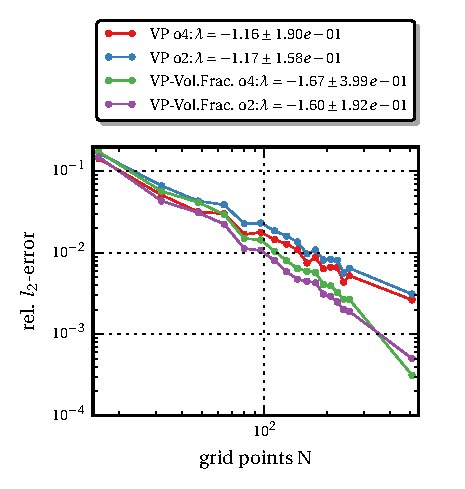
\includegraphics{gfx/immersed_boundary/hpflow/theo/vp.pdf}
      \caption{Relative $l_2$-error for different Volume-Penalization methods.}
  \end{minipage}
  \begin{minipage}[c]{0.5\textwidth}
      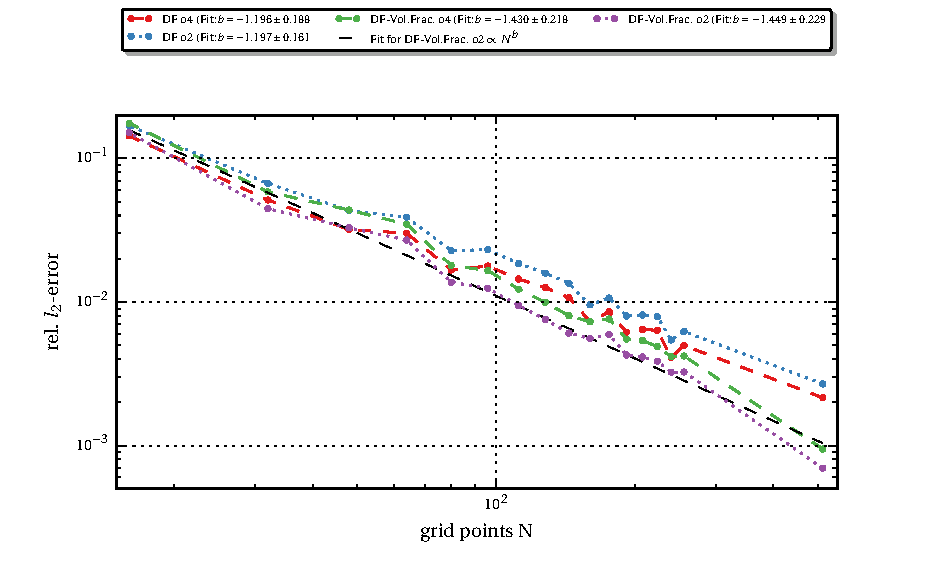
\includegraphics{gfx/immersed_boundary/hpflow/theo/df.pdf}
      \caption{Relative $l_2$-error for different Direct-Forcing methods.}
  \end{minipage}
  \begin{minipage}[c]{0.5\textwidth}
      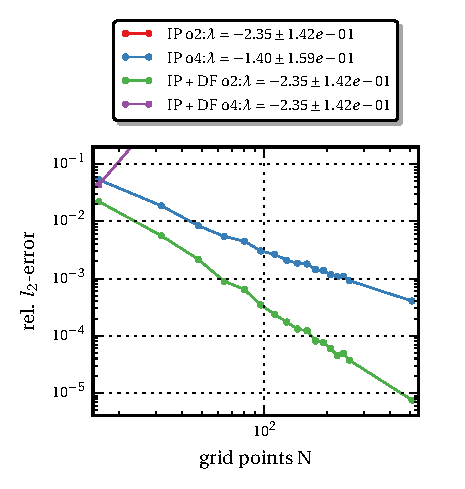
\includegraphics{gfx/immersed_boundary/hpflow/theo/ip.pdf}
      \caption{Relative $l_2$-error for different Interpolation methods.}
  \end{minipage}
  \begin{minipage}[c]{0.5\textwidth}
      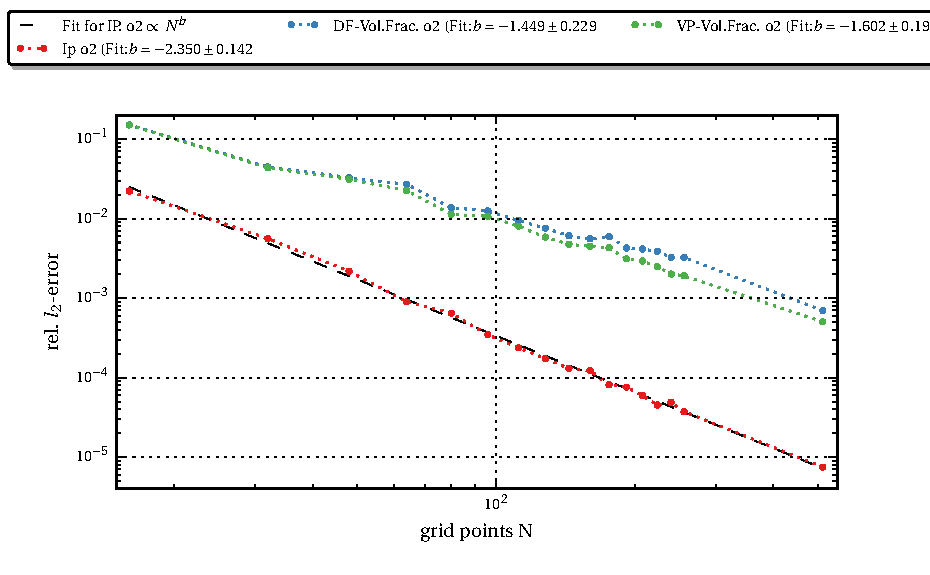
\includegraphics{gfx/immersed_boundary/hpflow/theo/all.pdf}
      \caption{Relative $l_2$-error for the methods with the smallest error in comparsion.}
  \end{minipage}
\end{figure}
\clearpage
\subsubsection{Grid Convergence Study with Comparsion to High Resolution Solution}


As we allready could observe in section (), each immersed boundary method does not converge against the exact theoretical solution.
Therefore, for each method, he theoretical solution is given by a
high resolution solution of each method with $N=512$ points.
This type of grid convergence study is often proposed
when no theoretical solution of the fluid problem can be achieved (SOURCE).
Here we use $N\in\{16, 32, 64, 128, 256\}$ for the number of grid points, for the comparision.

The problem occuring with other $N$ is the position of grid points, which would not exactly overlap anymore with
the high resolution grid  of the theoretical solution of $N=512$.
An alternative would be to use interpolation methods for the exact positions, but the possible disadvantage with these method
would be an additional error resulting from the interpolation scheme.\\

The results for this simulation will be discussed exemplarily for the Volume-Penalization method, the Direct-Forcing method with
use of the Volume-Fraction method and 2nd order, the Interpolation method, for 2nd and 4th order finite difference schemes.
Not all results are considered  because the computation contains an error, due to a false assumption.
This will be discussed in more detail in Sec. \ref{vali:hpflow_discussion}
The relative $l_2$-error of this simulations is shown in Fig. \ref{vali:hpflow_results_gchd_all}.

For the Direct-Forcing and Volume-Penalization methods the error convergence rate is about  $1.45$ and $1.6$.
The interpolation method with 4th order finite differences has a smaller decay about $1.4$, altough the overall error
is smaller.
The interpolation method with 2nd order has a decay about 2.35 and contains the smallest error.

In Fig. \ref{vali:hpflow_results_gchd_example} the difference between the theoretical profile from Eq. () and
the computed velocity profile for the Direct Forcing method is shown for a resolution of $N=256$.
It can be noticed that the error vanishes in the center of the fluid domain, but is large at the border
about ().



\begin{figure}[!bp]
  \begin{minipage}[c]{0.5\textwidth}
      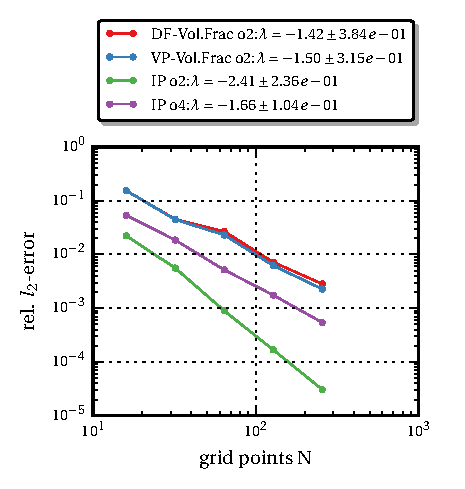
\includegraphics{gfx/immersed_boundary/hpflow/hd/all.pdf}
      \caption{\label{vali:hpflow_results_gchd_all}
          Relative $l_2$-error for the Volume-Penalization, Direct-Forcing  methods.}

  \end{minipage}
  \begin{minipage}[c]{0.5\textwidth}
      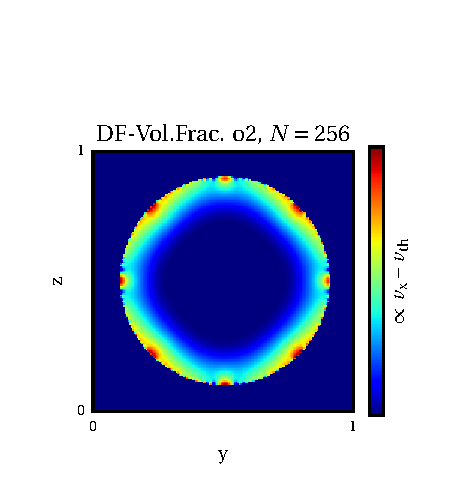
\includegraphics{gfx/immersed_boundary/hpflow/hd/example.pdf}
      \caption{\label{vali:hpflow_results_gchd_example}
        Exemplarily velocity difference .
         }
  \end{minipage}
\end{figure}

%The convergence rate of the volume penalization method and direct forcing method are of order $\approx 1.44$ and $\approx 1.6$.
%Since the finite difference methods are of 2nd order, one would expect a similar decrease in the error.
%However we can explain this behaviour by having a look at the velocity profile substracted from the theoretical solution.
%Fig. () (b) shows this exemplarly for the direct forcing volume fraction method. It can be noted that
%the error vanishes in the middle section of the fluid error whereas the largest differences occur at the fluid domain border.


\subsubsection{Long-Term Simulations}

The long-term simulations were performed in order to test the numerical-stability and the conservation of mass.
For all methods, except the IP-o4 method, the simulation were numerical stable.

For all o2 methods, the density averaged of the fluid domain is constant, which indicates that the total mass flux through the
boundaries has to be zero.
It can be seen that for all methods of o4 oscillations in the density emerge.
This is exemplariliy shown in Fig.  \ref{hpflow:results_long_ts} for the Direct-Forcing Vol.Frac. method of 4th order.
The profile of the other methods of o4, can be fonud in Appendix ().

Finally in Fig. \ref{hpflow:results_long_example} the averaged density with respect to the simulation time is shown for the
4th order methods.
For the default Direct-Forcing and Volume-Penalization methods the density increases to about $5\cdot10^{-5}$.
For methods with volume fraction the density decreases to bla.
ip bla

For all methods the a change in the average density can be observed, however
es gibt eine sättigung für alle verfahren spätestens bei 1600.
und die  wert ist eher klein.

\begin{figure}[!bp]
  \begin{minipage}[c]{0.5\textwidth}
      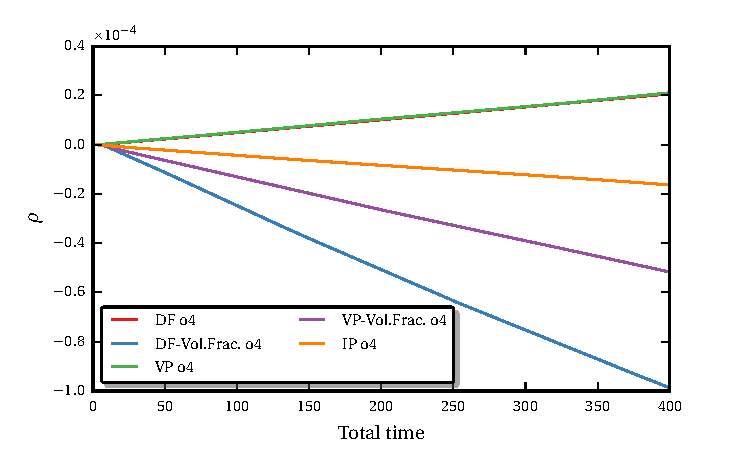
\includegraphics{gfx/immersed_boundary/hpflow/long/ts.pdf}
      \caption{\label{hpflow:results_long_ts}
            Averaged density with respect to the simulation time.
          }
  \end{minipage}
  \begin{minipage}[c]{0.5\textwidth}
      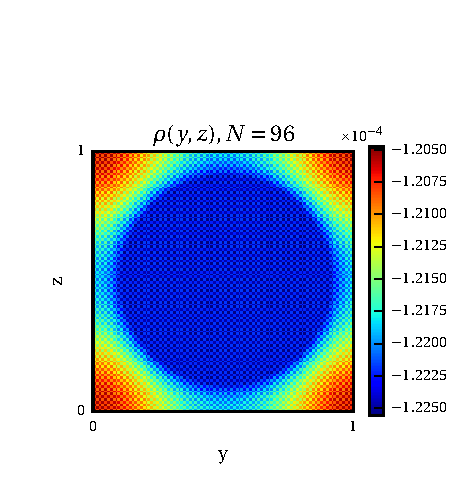
\includegraphics{gfx/immersed_boundary/hpflow/long/example.pdf}
      \caption{\label{hpflow:results_long_example}
        Density in the xy plane for$ z = 0.5 t = tend$.
      }
  \end{minipage}
\end{figure}


\clearpage

\subsection{Discussion}
\subsubsection{Grid Convergence Study}


-alle methoden except ip haben gleiche fehler ordnung
-fraction methdos is a little bit better
-the best error is interpolation

- ip o4 unstable mit mit DF o4 possible explanation is given in sec. .
- ip o2 identical to o4


 The identy of these methods occurs due to the decoupling of the velocity fields
on the border ot the fluid domain. Since the interpolation stencil seperates the fluid and wall domain, the 2nd order
stencil doesn't see any points in the wall domain, therefore there is no difference in using the direct forcing method.\\

\subsubsection{Grid Convergence Study with Comparsion to High Resolution Solution}
\label{vali:hpflow_discussion}

-different boundaries

Therefore we propose that the bad convergence is caused by different approximations of the wall region for different resolutions.
Since the boundary is not mimiced exactly but approximated by the nearest neighboor points in the wall domain, the actual position
of the boundary is dependent of the resolution.\\

-interpolation o2  comparison to paper with gc study

The interpolation method of 4th order converges with a rate of $\approx 1.4$ order. It is therefore even worse than the volume penalization and
direct forcing method, altough the overall error is smaller for lower resolutions. Again one possible explanation would be the different rasterization
of the domain border, which does not affect the velocity profiles due to the interpolation but the coupling of the pressure.\\
The 2nd order interpolation method converges is of order $\approx 2.35$, which is better than the expected order of two.
The fluid domain is interpolated at the same positions and since no pressure coupling over the fluid wall occurs the induced error is small.

\subsubsection{Long-Term Simulations}
-density changes
-a part goes into immersed boundary
-howerver the overall influence can be neglected


